\documentclass{article}
\usepackage[utf8]{inputenc}
\usepackage{graphicx}

\title{Software Design Document: Knowledge Expiration Tracker}
\author{Daniel Yang, Chad Wong, Raymond Diep, William Lopez, Liam Peak}
\date{May 12, 2026}

\begin{document}

\maketitle
\newpage
\tableofcontents
\newpage

\section{Versions Table}
\begin{tabular}{|l|l|l|l|}
\hline
\textbf{Version} & \textbf{Date} & \textbf{Description} & \textbf{Author} \\ \hline
1.0 & 05/12/2026 & Snapshot 1: Framework and Architecture & Group \\ \hline
\end{tabular}

\section{Introduction}
This document outlines the architectural design for the Knowledge Expiration Tracker, a containerized MERN/PERN stack application.

\section{System Architecture}
The system utilizes Docker Compose to orchestrate three primary services:
\begin{itemize}
    \item \textbf{Frontend:} A React.js application for the user interface.
    \item \textbf{Backend:} A Node.js and Express.js API for logic and auth.
    \item \textbf{Database:} A PostgreSQL instance for persistent storage.
\end{itemize}

\section{High-Level Workflow}
The following diagram illustrates the data flow between the user, the API, and the data storage layer:
% Note: Make sure workflow.png is uploaded to your GitHub repo
% 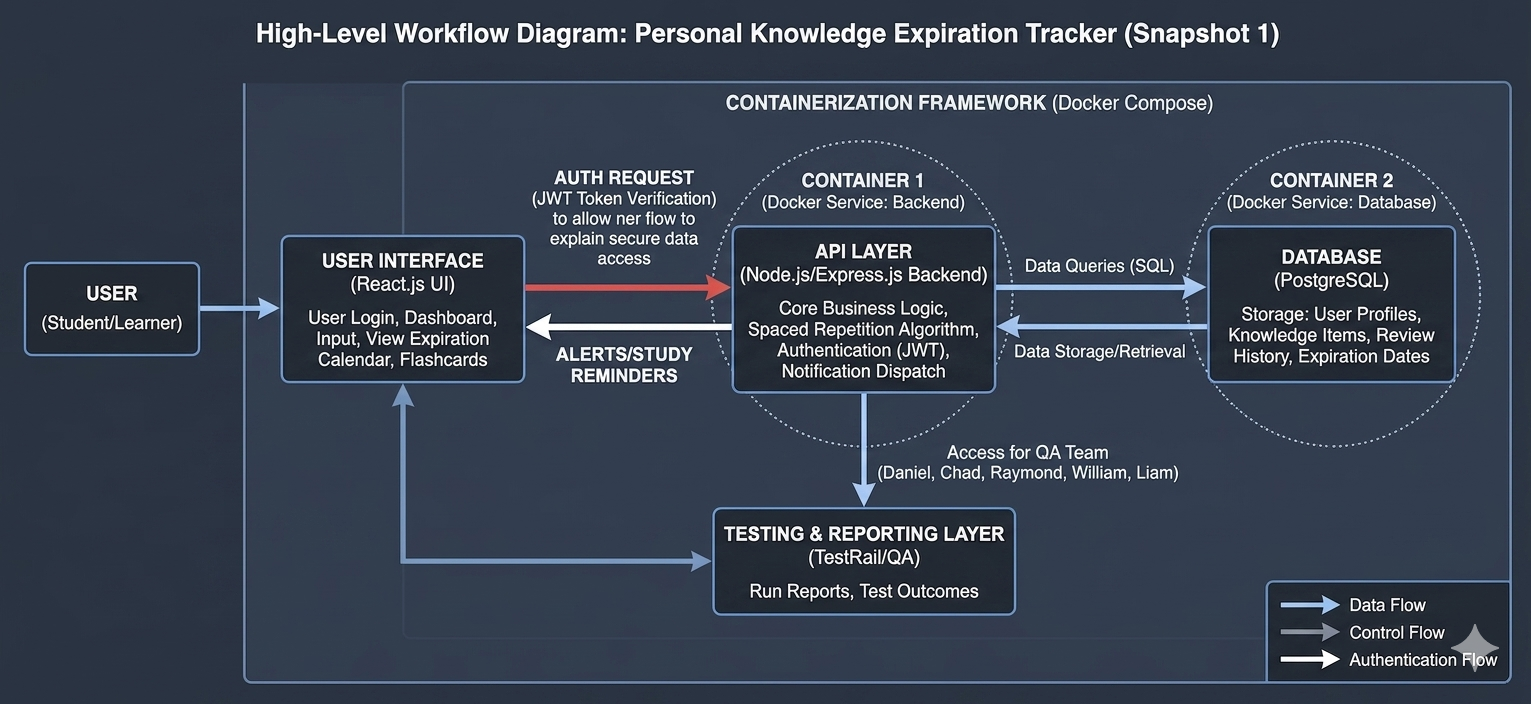
\includegraphics[width=\textwidth]{workflow.png}

\section{Glossary}
\begin{itemize}
    \item \textbf{Spaced Repetition:} A learning technique incorporating increasing intervals of time between reviews.
    \item \textbf{Docker:} A platform to create, deploy, and run applications in containers.
    \item \textbf{JWT (JSON Web Token):} An open standard for sharing security information.
    \item \textbf{Active Recall:} A principle of efficient learning involving memory stimulation.
\end{itemize}

\end{document}
